% !TeX spellcheck = en_GB
\documentclass{article}

\usepackage{float}
\usepackage[hidelinks]{hyperref}
\usepackage{graphicx}
\usepackage{caption}
\usepackage{tabu}
\usepackage{subcaption}
\usepackage{adjustbox}

\author{Anders Wind Steffensen (awis@itu.dk)\and Mikael Lindemann (mlin@itu.dk)\\\\Supervisor: Sebastian Risi (sebr@itu.dk)}
\title{Shortest Path in Undirected Unweighted Graphs using Evolvable Neural Turing Machine}

\begin{document}
\maketitle
\tableofcontents
\newpage
\section{Background}
\subsection{Graphs}
A \textit{graph} $G(V,E)$ is data-structure which consists of a set of \textit{vertices} $V$ and a set of \textit{edges} $E$ where an edge is a pair of vertices $(u,v)$. An \textit{undirected graph} implies that if edge $ (u,v) $ exists then $ (v,u) $ exists in the graph. An \textit{unweighted graph} every edge is equal in the cost to traverse it. 
Two vertices are \textit{adjacent} if they are part of the same edge $ e $. A \textit{path} $ P $ is a ordered set of edges such that every consecutive edge shares a vertex. To vertices $ u $, $ v $ are \textit{connected} if there exist a path between $ u $, $ v $.

In an undirected unweighted graph the length of a path P is $ |P| $. A shortest path between two vertices  $ u $, $ v $ is a path $ P $ connecting  $ u $, $ v $ of the smallest length. 

\subsection{Neural Networks}
A \textit{neural network} is an approximation method for n dimensional functions. Neural networks consists of a collection of \textit{layers} $ L_1 .. L_n $ where $ L_1 $ is the \textit{input layer} and $ L_2 ... L_{n-1} $ are \textit{hidden layers} and $ L_n $ is the \textit{output layer}. Each layer $ Li $ consist of a number of \textit{neurons}. A neuron is connected to other neurons in the layer before and after its own layer. Neurons can send signals to other neurons it is connected to. The strength of a signal is specified by a \textit{signal function} of a neuron. Neurons gets \textit{activated} and sends a signal if itself has become activated a \textit{threshold} amount by other neurons. The signal function is based on a \textit{formula}, a \textit{weight} and a \textit{bias}. 

The \textit{feed forward algorithm} activates the neurons of the input layer based on some input data, whom in return activates the neurons of the next layer and so on. The values of the output layer is then read. The \textit{backpropagation algorithm} calculates the error of the output neurons compared to the input data and corrects it based on a function. The errors or then backpropagated through the layers. By running the feed forward and backpropagation algorithms in combination with enough data, almost any function can be approximated.

A \textit{one hot encoding} of a nominal data point, is a conversion of the data point into a bit array $ A $ with the length of the range of possible nominal values. For a nominal value $ i $ only $ A[i] $ is $ 1 $.  

\subsection{Evolutionary Neural Networks}

\subsubsection{NeuroEvolution of Augmenting Topologies (NEAT)}

\subsection{Evolvable Neural Turing Machine}

\section{Experiment}
Given an unweighted undirected graph $G$, a source vertex $s$, and a target vertex $t$, find the shortest path from $s$ to $t$ in $G$.

We have restricted the problem to instances where a path between $s$ and $t$ exists.

\subsection{Instance encoding}
In order to feed the instance into the network, we use a one hot encoding of the adjacency matrix of the graph and each of the source and target vertices. See \autoref{fig:input:encoding} for an example.

\begin{figure}[hb]
	\centering
	\begin{subfigure}{.5\textwidth}
		\centering
		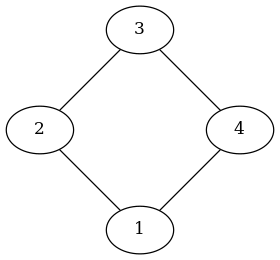
\includegraphics[scale=.5]{figures/encoding.png}
	\end{subfigure}%
	\begin{subfigure}{.5\textwidth}
		\centering
		\begin{tabular}{|c|c|c|c|c|}
			\hline
			&\textbf{1}&\textbf{2}&\textbf{3}&\textbf{4}\\\hline
			\textbf{1}&0&1&0&0\\\hline
			\textbf{2}&1&0&1&1\\\hline
			\textbf{3}&0&1&0&1\\\hline
			\textbf{4}&0&1&1&0\\\hline
		\end{tabular}
	\end{subfigure}\par\bigskip
	\begin{adjustbox}{center}
		\begin{subfigure}{1.3\textwidth}
			\centering
			\begin{tabu}{|c|c|c|c||c|c|c|c||c|c|c|c||c|c|c|c|[2pt]c|c|c|c|[2pt]c|c|c|c|}
				\hline
				0&1&0&0&1&0&1&1&0&1&0&1&0&1&1&0&1&0&0&0&0&0&0&1\\\hline
			\end{tabu}
		\end{subfigure}
	\end{adjustbox}
	\caption{Shows a simple graph, its adjancency matrix and an encoding where $s=1$ and $t=4$. Thick lines between cells means encoding of a new structure. The three structures are the flattened adjacency table, with each row delimited with double lines for visibility, the one-hot encoding of $s$, and the one-hot encoding of $t$}
	\label{fig:input:encoding}
\end{figure}

When the neural network using the turing machine returns output, this is a one-hot encoding of the next vertex on the path to the target.

This means that we can run the graph through the neural network multiple times, and each time, the neural network will tell us which vertex to move to, which we can give it back as the new source vertex to move from.

\section{Results}
\section{Conclusion}
\end{document}
